\documentclass{standalone}
\usepackage{xcolor}
\usepackage{verbatim}
\usepackage[T1]{fontenc}
\usepackage{graphics}
\usepackage{hyperref}
\newcommand{\code}[1]{\texttt{#1}}
\newcommand{\R}{R}
\newcommand{\pkg}[1]{#1}
\newcommand{\CRANpkg}[1]{\pkg{#1}}%
\newcommand{\BIOpkg}[1]{\pkg{#1}}
\usepackage{amsmath,amssymb,array}
\usepackage{booktabs}
\usepackage[english]{babel}
\usepackage{subcaption}
\usepackage{amsfonts}
\usepackage{bbm}
\usepackage{tikz}
\usetikzlibrary{automata,positioning}
\usepackage{bm}
\newcommand\codeNew{\bgroup\@makeother\_\@makeother\~\@makeother\$\@codex}

\begin{document}
\nopagecolor
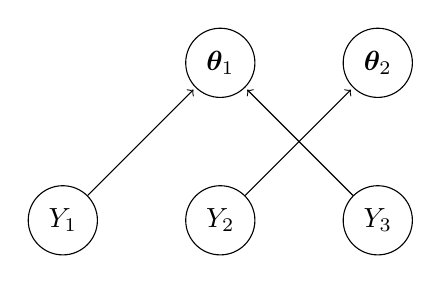
\begin{tikzpicture}[shorten >=1pt,node distance=2cm,on grid,auto]
		\node[state] (y1)  {$Y_1$}; 
		\node[state] (y2) [right=of y1] {$Y_2$}; 
		\node[state] (y3) [right=of y2] {$Y_3$}; 
		\node[state] (theta_1) [above=of y2] {${\bm\theta_1}$};
		\node[state] (theta_2) [above=of y3] {${\bm\theta_2}$};
		\path[->]
		(y1) edge node {} (theta_1)
		(y2) edge node {} (theta_2)
		(y3) edge node {} (theta_1);
		\end{tikzpicture} 
\end{document}
